\documentclass{beamer}
\usetheme{Madrid}
\usecolortheme{default}

\usepackage{listings}
\lstset{
  language=Haskell,
  basicstyle=\ttfamily,
  keywordstyle=\color{blue},
  commentstyle=\color{green!40!black},
  stringstyle=\color{orange},
  showstringspaces=false,
  breaklines=true,
  frame=single,
  numbers=left,
  numberstyle=\tiny,
  numbersep=5pt,
  xleftmargin=10pt,
}

%Information to be included in the title page:
\title[Functional Pearl - Russo] %optional
{Functional Pearl: \newline Two Can Keep a Secret, If One of Them Uses Haskell}
\subtitle{}
\author[Ines Cipullo] % (optional, for multiple authors)
{Alejandro Russo}
\institute[LCC - FCEIA] % (optional)
{
  Facultad de Ciencias Exactas, Ingeniería y Agrimensura,\\
  Universidad Nacional de Rosario.
}
\date[]{Ines Cipullo - Diciembre 2024}

\begin{document}

\frame{
    \titlepage
}

\section{Introducción}
\subsection{Ejemplo motivacional}

\begin{frame}
\frametitle{Ejemplo motivacional}
    Código de Alice para seleccionar contraseñas:
    \begin{center}
        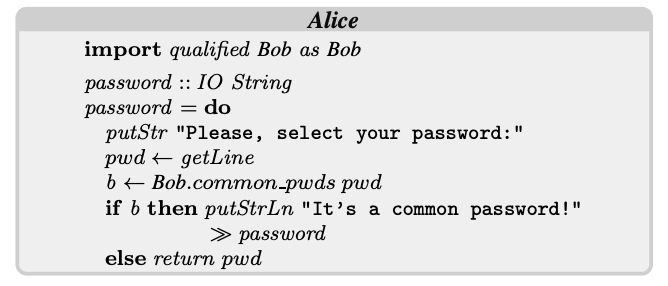
\includegraphics[scale=0.7]{codigo_alice.png}
    \end{center}

    Código malicioso de Bob:
    \begin{center}
        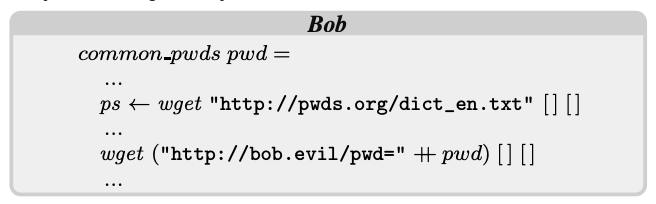
\includegraphics[scale=0.7]{codigo_bob.png}
    \end{center}
\end{frame}

\begin{frame}
\frametitle{Ejemplo motivacional}
    ¿Qué debería hacer Alice?
    \vspace{0.7cm}
    
    Proteger secretos no se trata de poner recursos en una lista negra (o blanca), sino de asegurar que la información fluye solo hacia los lugares adecuados.
    \vspace{0.7cm}
    
    \pause
    ¿Cómo se logra eso?
\end{frame}

\subsection{MAC e IFC}

\begin{frame}
    \frametitle{Mandatory Access Control e Information-Flow Control}
    \begin{itemize}
        \item<1-> Las técnicas de MAC e IFC asocian datos con etiquetas de seguridad para definir su nivel de confidencialidad.
        \item<1-> MAC proviene de la investigación de sistemas operativos, mientras que IFC proviene de la comunidad de los lenguajes de programación.
        \item<1-> ¿Qué propone esta funcional pearl? 
        
        Busca cerrar la brecha entre MAC e IFC al aprovechar conceptos de lenguajes de programación para implementar mecanismos similares a MAC mediante la creación de una API monádica que protege confidencialidad estáticamente.
    \end{itemize}
\end{frame}

\section{\textbf{MAC}}

\subsection{Modelado}

\begin{frame}{Látices de seguridad}
    ¿Cómo se etiquetan los datos?
    
    Formalmente las etiquetas están organizadas en un látice de seguridad.

    \begin{center}
        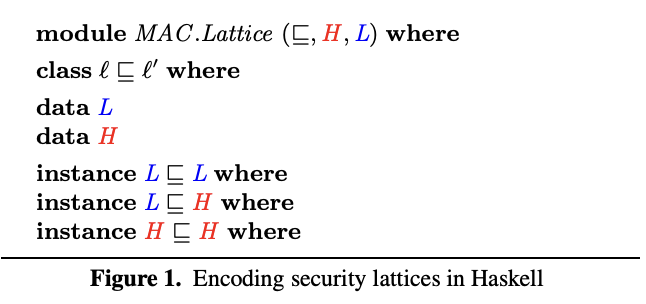
\includegraphics[scale=0.8]{figure1.png}
    \end{center}

    La información no puede fluir de entidades secretas a entidades públicas (no interferencia): $L \sqsubseteq H$ y $H \not\sqsubseteq L$.

\end{frame}

\begin{frame}{Familia de mónadas \textit{MAC}}
    Se introduce la familia de mónadas \textit{MAC}, que encapsula acciones de \textit{IO} y restringe su ejecución a situaciones donde la confidencialidad no se ve comprometida. 

    Está indexada por una etiqueta de seguridad indicando la sensibilidad de sus resultados monádicos. 

    \begin{center}
        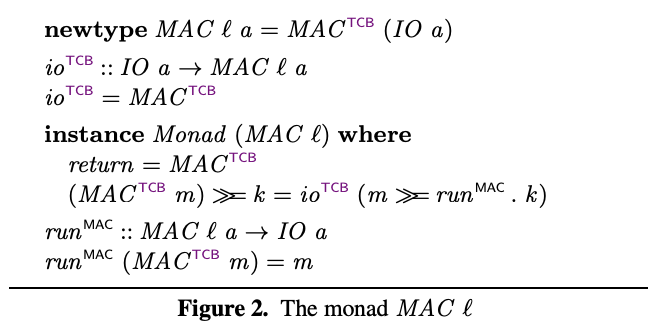
\includegraphics[scale=0.7]{figure2.png}
    \end{center}
\end{frame}

\begin{frame}{Recursos etiquetados}
    
    \begin{center}
        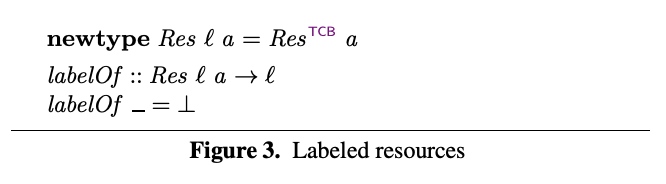
\includegraphics[scale=0.7]{figure3.png}
    \end{center}

    \begin{center}
        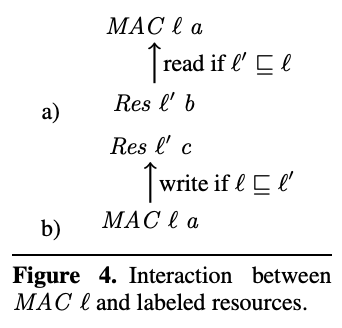
\includegraphics[scale=0.7]{figure4.png}
    \end{center}
\end{frame}

\begin{frame}{Lift de las acciones de IO}
    Siguiendo los principios de \textit{no read-up} y \textit{no write-down} se extiende la TCB con funciones que elevan las acciones \textit{IO}.

    \begin{center}
        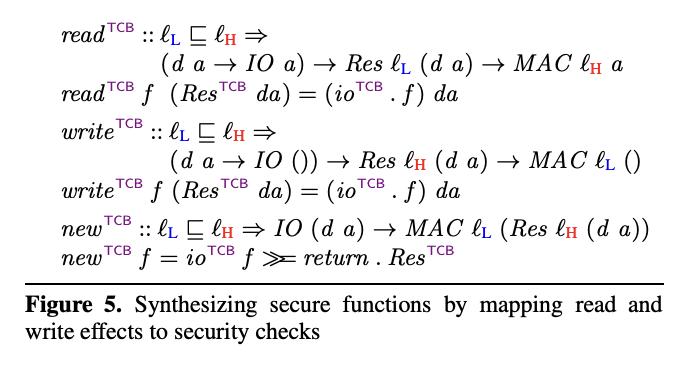
\includegraphics[scale=0.7]{figure5.png}
    \end{center}
\end{frame}

\begin{frame}{Expresiones etiquetadas}
    \begin{center}
        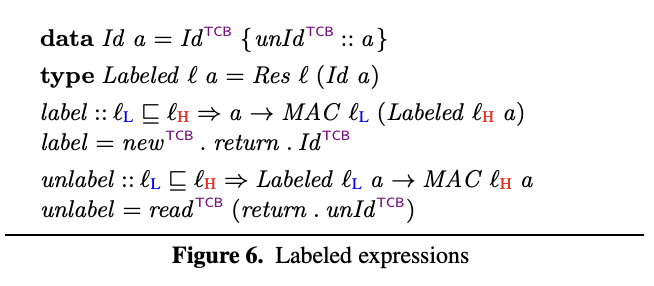
\includegraphics[scale=0.8]{figure6.png}
    \end{center}
\end{frame}

\begin{frame}[fragile]
    \frametitle{Uniendo miembros de la familia}
    Continuando con el ejemplo, si Bob usase \textit{MAC} su función podría tener el tipo

    \begin{lstlisting}
common_pwds :: Labeled H String -> MAC L (MAC H Bool)
    \end{lstlisting}
    
    En este caso la anidación de computaciones es manejable, pero habrá casos para los que tal vez no, por eso se introduce:

    \begin{center}
        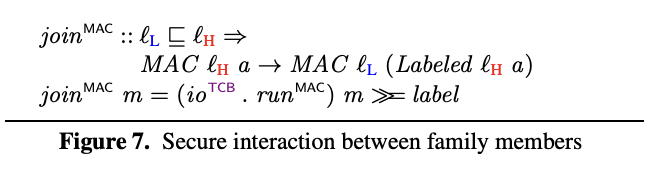
\includegraphics[scale=0.8]{figure7.png}
    \end{center}
\end{frame}

\subsection{Estructuras mutables: añadiendo referencias}

\begin{frame}{Añadiendo referencias}
    \begin{center}
        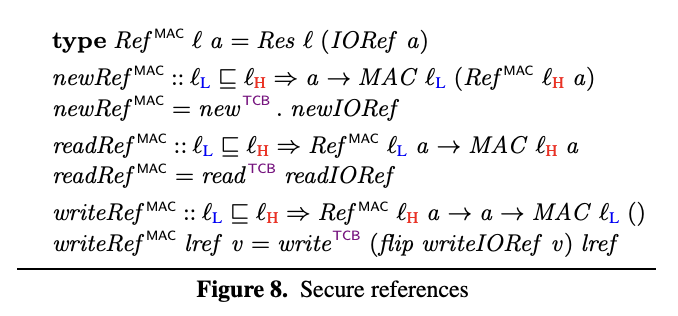
\includegraphics[scale=0.7]{figure8.png}
    \end{center}

    Las funciones se elevan a la mónada $MAC \ l$ envolviéndolas con $new^{TCB}$, $read^{TCB}$ y $write^{TCB}$ respectivamente. 

    Estos pasos se generalizan para obtener interfaces seguras de diversos tipos, como veremos más adelante.
\end{frame}

\subsection{Manejo de errores}

\begin{frame}{Añadiendo excepciones}
    \begin{center}
        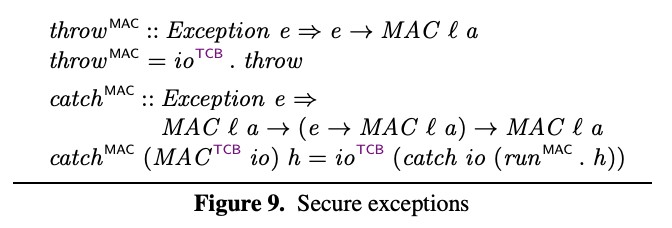
\includegraphics[scale=0.7]{figure9.png}
    \end{center}

    Podemos notar que las excepciones se capturan en el mismo tipo de miembro de la familia donde fueron arrojadas.

    Pero, ¿qué pasa con las construcciones con $join^{MAC}$?
    
    Pueden comprometer la seguridad.
    
    Una acción de nivel alto puede lanzar excepciones y evitar acciones de nivel bajo con la función $join^{MAC}$.
\end{frame}

\begin{frame}{Bob vuelve al ataque}

    \begin{center}
        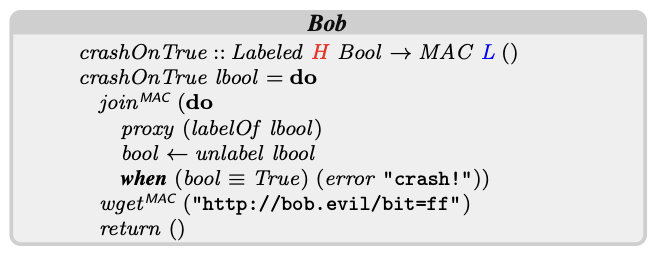
\includegraphics[scale=0.7]{codigo_bob2.png}
    \end{center}

    \begin{center}
        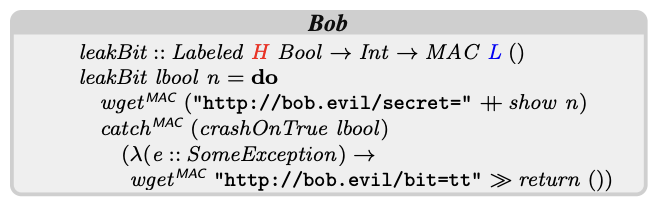
\includegraphics[scale=0.7]{codigo_bob3.png}
    \end{center}
\end{frame}

\begin{frame}{Nuevo $join^{MAC}$}
    Se redefine $join^{MAC}$ de manera tal que la propagación de excepciones entre miembros de la familia quede deshabilitada.

    \begin{center}
        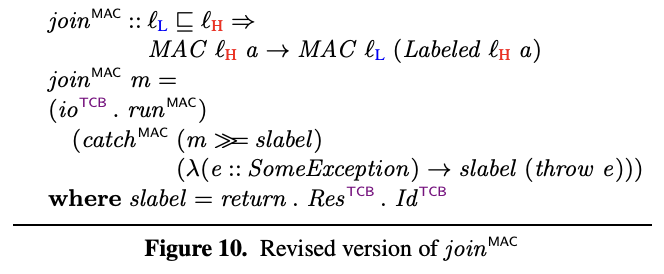
\includegraphics[scale=0.7]{figure10.png}
    \end{center}
\end{frame}

\subsection{El elefante (encubierto) en la habitación}
\begin{frame}{El elefante (encubierto) en la habitación}
    Existe un canal encubierto: la no terminación de programas.

    \vspace{0.5cm}
    En un entorno secuencial, la manera más efectiva de explotar un canal encubierto de no-terminación es a través de fuerza bruta, por lo que no hay gran ancho de banda si el universo donde buscar es lo suficientemente grande y en ese caso se puede omitir el análisis de estos canales encubiertos.

    \vspace{0.5cm}
    \pause
    ¿Pero qué sucede cuando hay concurrencia?
\end{frame}

\subsection{Concurrencia}

\begin{frame}{Bob con concurrencia}
    Alice añade concurrencia extendiendo la API así:

    \begin{center}
        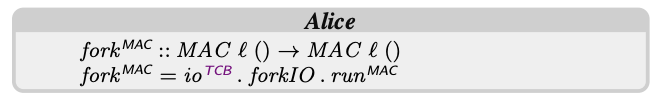
\includegraphics[scale=0.8]{codigo_alice2.png}
    \end{center}

    Y ahora Bob puede tomarse el trabajo de intentar explotar el canal encubierto de la no terminación de programas.
\end{frame}

\begin{frame}{Bob con concurrencia}
    \begin{center}
        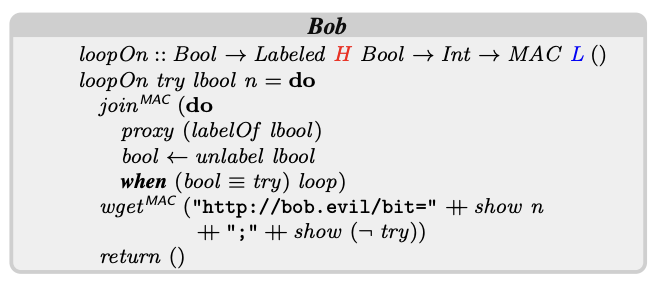
\includegraphics[scale=0.7]{codigo_bob4.png}
    \end{center}

    \begin{center}
        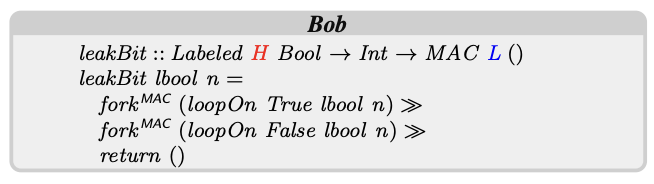
\includegraphics[scale=0.7]{codigo_bob5.png}
    \end{center}
\end{frame}

\begin{frame}{Solución}
    El problema viene de la interacción de $join^{MAC}$ con $fork^{MAC}$.

    Pero, ¡se puede reemplazar a $join^{MAC}$ por $fork^{MAC}$!

    \begin{center}
        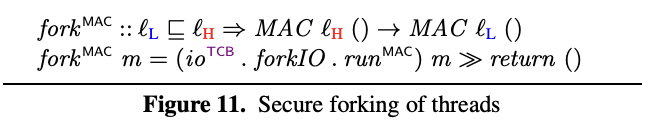
\includegraphics[scale=0.8]{figure11.png}
    \end{center}

    Aunque se haya removido $join^{MAC}$ se pueden combinar computaciones con las referencias seguras introducidas previamente.
\end{frame}

\begin{frame}{MVars}
    Se extiende \textbf{MAC} con \textit{MVars} ---una abstracción de sincronización muy utilizada en Haskell--- de manera muy similar a como se hizo con referencias.
    
    \begin{center}
        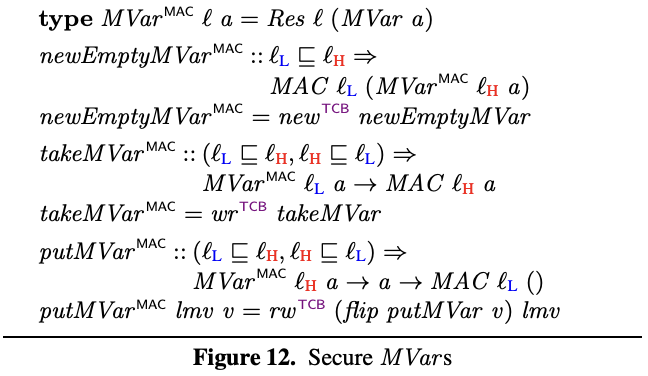
\includegraphics[scale=0.8]{figure12.png}
    \end{center}
\end{frame}

\section{Comentarios finales}

\begin{frame}{Comentarios finales}
    \begin{itemize}
        \item<1-> Las abstracciones que provee Haskell y, en general, los lenguajes funcionales, son muy amenas para enfrentarse a los desafíos de seguridad actuales.

        \item<2-> La correción de \textbf{MAC} depende de la seguridad de tipos y la encapsulación de módulos de Haskell. GHC incluye características y extensiones del lenguaje capaces de romper ambas características. Safe Haskell (Terei et al. 2012) es una extensión de GHC que identifica un subconjunto de Haskell que sigue la seguridad de tipos y la encapsulación de módulos. MAC utiliza Safe Haskell al compilar código no confiable.
    \end{itemize}
\end{frame}

% References (needs a .bib file)
% \begin{frame}{Fuentes}
% \nocite{*}
% \bibliographystyle{plain}
% \bibliography{ref}
% \end{frame}

\end{document}